\documentclass[aspectratio=169]{beamer}
\usepackage{amsmath}
\usepackage{amssymb}
\usepackage{tikz}
\usepackage{xcolor}
\usetikzlibrary{shapes,backgrounds,patterns}

\usepackage{pgfplots}
\pgfplotsset{compat=1.18, legend cell align=left}
\usetikzlibrary{arrows.meta,decorations.pathreplacing,calc,positioning}
\usepackage{booktabs}

% royalblue isn't a base xcolor name, so define it first (this is the default accent)
\definecolor{royalblue}{RGB}{65,105,225}

% ============================================================
%  ACCENT COLOR: change ONE line below to switch the theme
%  Choose one of: royalblue , red , black
% ============================================================
\colorlet{accent}{royalblue}
% \colorlet{accent}{red}
% \colorlet{accent}{black}
% ============================================================

% colorblind-safe, high-contrast second color (Okabe-Ito vermillion)
\definecolor{hl}{RGB}{213,94,0}
% third curve color (Okabe-Ito bluish green)
\definecolor{gr}{RGB}{0,158,115}

\usetheme{default}
\setbeamercolor{background canvas}{bg=white}
\setbeamercolor{normal text}{fg=black}
\setbeamercolor{structure}{fg=accent}
\setbeamercolor{frametitle}{fg=accent,bg=white}
\setbeamercolor{title}{fg=accent}
\setbeamercolor{section in toc}{fg=black}
\setbeamercolor{block title}{fg=black,bg=gray!10}
\setbeamercolor{block body}{fg=black,bg=gray!5}
\setbeamercolor{block title example}{fg=black,bg=green!10}
\setbeamercolor{block body example}{fg=black,bg=green!5}
\setbeamercolor{block title alerted}{fg=black,bg=red!10}
\setbeamercolor{block body alerted}{fg=black,bg=red!5}

\setbeamertemplate{navigation symbols}{}
\setbeamertemplate{footline}{
    \hfill\makebox[5pt]{%
        \scriptsize\insertframenumber}
    \hspace*{2em}
    \vspace{0.5cm}
}

\newcommand{\cbox}[2]{\colorbox{#1}{\ensuremath{\displaystyle #2}}}

\title{Interpolation in 2-D: The Ideas Behind the Code}
\subtitle{Grids, scattered data, and the convex hull}
\author{Sharareh Sayyad}
\institute{Washington State University}
\date{\today}


\begin{document}

\frame{\titlepage}

% ============================================================
% 1. Two situations
% ============================================================
\begin{frame}{From curves to surfaces}
\begin{columns}[c]
\begin{column}{0.46\textwidth}
\small
\begin{block}{The task}
\footnotesize
given $(x_i, y_i, z_i)$, find $p$ with \cbox{accent!12}{p(x_i, y_i) = z_i}
\end{block}
The data come in \textbf{two shapes}:
\begin{itemize}
  \setlength{\itemsep}{2pt}
  \item \textbf{On a grid:} a value at every pair $(x_i, y_j)$.\\
  \footnotesize tables, images, simulation output
  \small
  \item \textbf{Scattered:} values at points with no pattern.\\
  \footnotesize sensors, weather stations
\end{itemize}
\vspace{0.1cm}
\begin{exampleblock}{The first question}
\footnotesize
Grid or scattered? The answer decides the method.
\end{exampleblock}
\end{column}
\begin{column}{0.52\textwidth}
\centering
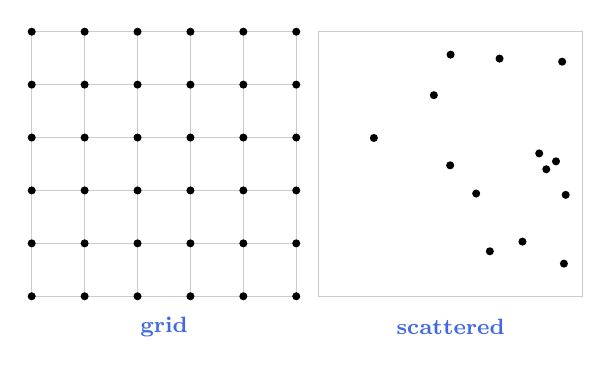
\begin{tikzpicture}[scale=0.56]
  \draw[gray!40, step=1.2] (0,0) grid (6,6);
  \foreach \i in {0,1.2,...,6.1} \foreach \j in {0,1.2,...,6.1} \fill[black] (\i,\j) circle (2.6pt);
  \node[accent, font=\footnotesize\bfseries] at (3,-0.7) {grid};
  \begin{scope}[xshift=6.5cm]
    \draw[gray!40] (0,0) rectangle (6,6);
    \foreach \p in {(5.39,3.06),(5.57,0.74),(3.58,2.33),(4.63,1.24),(5.01,3.24),(5.17,2.88),(2.62,4.56),(5.61,2.30),(5.53,5.32),(1.26,3.59),(4.11,5.39),(3.89,1.02),(2.99,2.97),(3.00,5.48)} \fill[black] \p circle (2.6pt);
    \node[accent, font=\footnotesize\bfseries] at (3,-0.7) {scattered};
  \end{scope}
\end{tikzpicture}\\[4pt]
\footnotesize A grid has \textbf{structure} we can use; scattered points do not.
\end{column}
\end{columns}
\end{frame}

% ============================================================
% 2. Grid
% ============================================================
\begin{frame}{Data on a grid: one direction at a time}
\begin{columns}[c]
\begin{column}{0.46\textwidth}
\small
A grid point lies in a \textbf{rectangle} of data.
\vspace{0.15cm}
\begin{block}{Tensor product idea}
\footnotesize
\textbf{1.} Interpolate along $x$ on the grid lines above and below.\\[2pt]
\textbf{2.} Interpolate along $y$ between those two values.
\end{block}
\vspace{0.05cm}
\begin{exampleblock}{Consequence}
\footnotesize
Every 1-D method carries over: \textbf{linear, cubic, PCHIP}.\\
Each keeps its 1-D character: local or global, safe or smooth.
\end{exampleblock}
\scriptsize
\texttt{si.RegularGridInterpolator((x, y), Z, method=...)}
\end{column}
\begin{column}{0.52\textwidth}
\centering
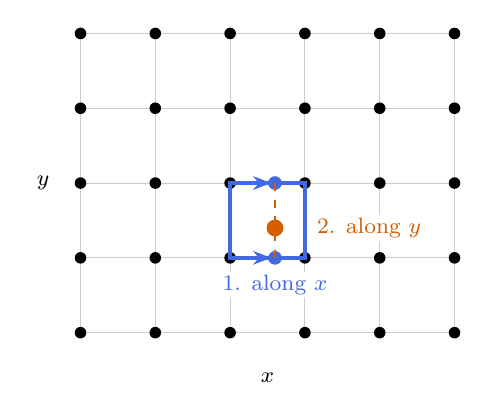
\begin{tikzpicture}[scale=0.95]
  \draw[gray!40] (0,0) grid (5,4);
  \foreach \i in {0,...,5} \foreach \j in {0,...,4} \fill[black] (\i,\j) circle (2.2pt);
  % the cell
  \draw[accent, very thick] (2,1) rectangle (3,2);
  % step 1
  \draw[accent, thick, -{Stealth}] (2,1) -- (2.55,1);
  \draw[accent, thick, -{Stealth}] (2,2) -- (2.55,2);
  \fill[accent] (2.6,1) circle (2.6pt);
  \fill[accent] (2.6,2) circle (2.6pt);
  % step 2
  \draw[hl, thick, dashed] (2.6,1) -- (2.6,2);
  \fill[hl] (2.6,1.4) circle (3.2pt);
  \node[accent, font=\footnotesize, anchor=north, fill=white, inner sep=1pt] at (2.6,0.82) {1. along $x$};
  \node[hl, font=\footnotesize, anchor=west, fill=white, inner sep=1pt] at (3.12,1.4) {2. along $y$};
  \node[font=\footnotesize] at (2.5,-0.6) {$x$};
  \node[font=\footnotesize] at (-0.5,2) {$y$};
\end{tikzpicture}\\[4pt]
\footnotesize The grid tells us at once which rectangle a point is in.
\end{column}
\end{columns}
\end{frame}

% ============================================================
% 3. Scattered data and the convex hull
% ============================================================
\begin{frame}{Scattered data: triangles and the convex hull}
\begin{columns}[c]
\begin{column}{0.46\textwidth}
\small
No grid, so we build our own cells: \textbf{triangles} with the data points as corners.
\vspace{0.15cm}
\begin{block}{Interpolate on each triangle}
\footnotesize
A new point lies in one triangle; use its \textbf{3 corners} (linear or cubic).\\
Local: far-away points do not matter.
\end{block}
\begin{alertblock}{The convex hull}
\footnotesize
The triangles cover only the \textbf{convex hull}: the smallest convex region holding all the points.\\
Outside it there is no triangle, so no answer (\texttt{nan}).
\end{alertblock}
\scriptsize
\texttt{si.griddata(pts, z, (Xn, Yn), method=...)}
\end{column}
\begin{column}{0.52\textwidth}
\centering
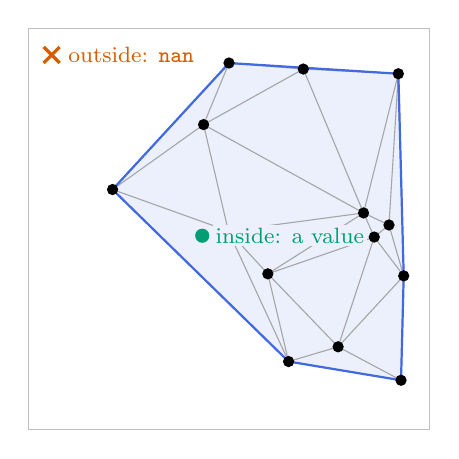
\begin{tikzpicture}[scale=0.85]
  \fill[accent!10] (3.00,5.48)--(1.26,3.59)--(3.89,1.02)--(5.57,0.74)--(5.61,2.30)--(5.53,5.32)--cycle;
  \begin{scope}[gray!70, thin]
  \draw (2.62,4.56)--(2.99,2.97); \draw (4.63,1.24)--(5.61,2.30); \draw (5.01,3.24)--(2.62,4.56); \draw (5.01,3.24)--(2.99,2.97); \draw (5.17,2.88)--(5.61,2.30); \draw (5.39,3.06)--(5.17,2.88); \draw (1.26,3.59)--(3.89,1.02); \draw (5.39,3.06)--(5.53,5.32); \draw (3.58,2.33)--(5.17,2.88); \draw (3.58,2.33)--(3.89,1.02); \draw (5.57,0.74)--(4.63,1.24); \draw (5.01,3.24)--(5.17,2.88); \draw (5.01,3.24)--(5.53,5.32); \draw (5.39,3.06)--(5.61,2.30); \draw (3.58,2.33)--(5.01,3.24); \draw (1.26,3.59)--(3.00,5.48); \draw (5.39,3.06)--(5.01,3.24); \draw (5.57,0.74)--(3.89,1.02); \draw (2.62,4.56)--(3.00,5.48); \draw (2.62,4.56)--(4.11,5.39); \draw (4.63,1.24)--(5.17,2.88); \draw (4.63,1.24)--(3.89,1.02); \draw (5.01,3.24)--(4.11,5.39); \draw (1.26,3.59)--(2.99,2.97); \draw (5.53,5.32)--(4.11,5.39); \draw (4.11,5.39)--(3.00,5.48); \draw (3.89,1.02)--(2.99,2.97); \draw (5.53,5.32)--(3.00,5.48); \draw (3.58,2.33)--(4.63,1.24); \draw (5.57,0.74)--(5.61,2.30); \draw (3.58,2.33)--(2.99,2.97); \draw (2.62,4.56)--(1.26,3.59); \draw (5.61,2.30)--(5.53,5.32);
  \end{scope}
  \draw[accent, thick] (3.00,5.48)--(1.26,3.59)--(3.89,1.02)--(5.57,0.74)--(5.61,2.30)--(5.53,5.32)--cycle;
  \foreach \p in {(5.39,3.06),(5.57,0.74),(3.58,2.33),(4.63,1.24),(5.01,3.24),(5.17,2.88),(2.62,4.56),(5.61,2.30),(5.53,5.32),(1.26,3.59),(4.11,5.39),(3.89,1.02),(2.99,2.97),(3.00,5.48)} \fill[black] \p circle (2.4pt);
  \fill[gr] (2.6,2.9) circle (3pt);
  \node[gr, font=\footnotesize, anchor=west, fill=accent!10, inner sep=1pt] at (2.75,2.9) {inside: a value};
  \draw[hl, very thick] (0.35,5.6) ++(-0.12,-0.12) -- ++(0.24,0.24) ++(-0.24,0) -- ++(0.24,-0.24);
  \node[hl, font=\footnotesize, anchor=west, fill=white, inner sep=1pt] at (0.55,5.6) {outside: \texttt{nan}};
  \draw[gray!50] (0,0) rectangle (6,6);
\end{tikzpicture}\\[2pt]
\footnotesize Blue outline: the convex hull. Shaded: where we can interpolate.
\end{column}
\end{columns}
\end{frame}

% ============================================================
% 4. Big picture
% ============================================================
\begin{frame}{The big picture}
\small
\centering
\setlength{\tabcolsep}{5pt}
\renewcommand{\arraystretch}{1.4}
\footnotesize
\begin{tabular}{llll}
\toprule
\textbf{Data} & \textbf{Cells} & \textbf{Where it answers} & \textbf{Tool} \\
\midrule
grid      & rectangles of the grid     & the whole grid       & \texttt{RegularGridInterpolator} \\
scattered & triangles between points   & the convex hull only & \texttt{griddata} \\
scattered & none: one smooth function  & everywhere           & \texttt{RBFInterpolator} \\
\bottomrule
\end{tabular}
\vspace{0.4cm}
\raggedright
\begin{block}{Take-home messages}
\footnotesize
\begin{enumerate}
  \setlength{\itemsep}{3pt}
  \item First ask: \textbf{grid or scattered?}
  \item On a grid, 2-D = \textbf{1-D along $x$, then along $y$}; the same trade-off: \textbf{smooth vs local}.
  \item Scattered data live on \textbf{triangles}; outside the \textbf{convex hull} there is no data.
  \item A method that answers outside the data (RBF) is \textbf{extrapolating}: trust values near the data.
\end{enumerate}
\end{block}
\end{frame}

\end{document}
